\subsection{Versuchsaufbau}
\label{sec:Versuchsaufbau}
\begin{figure}
	\centering
	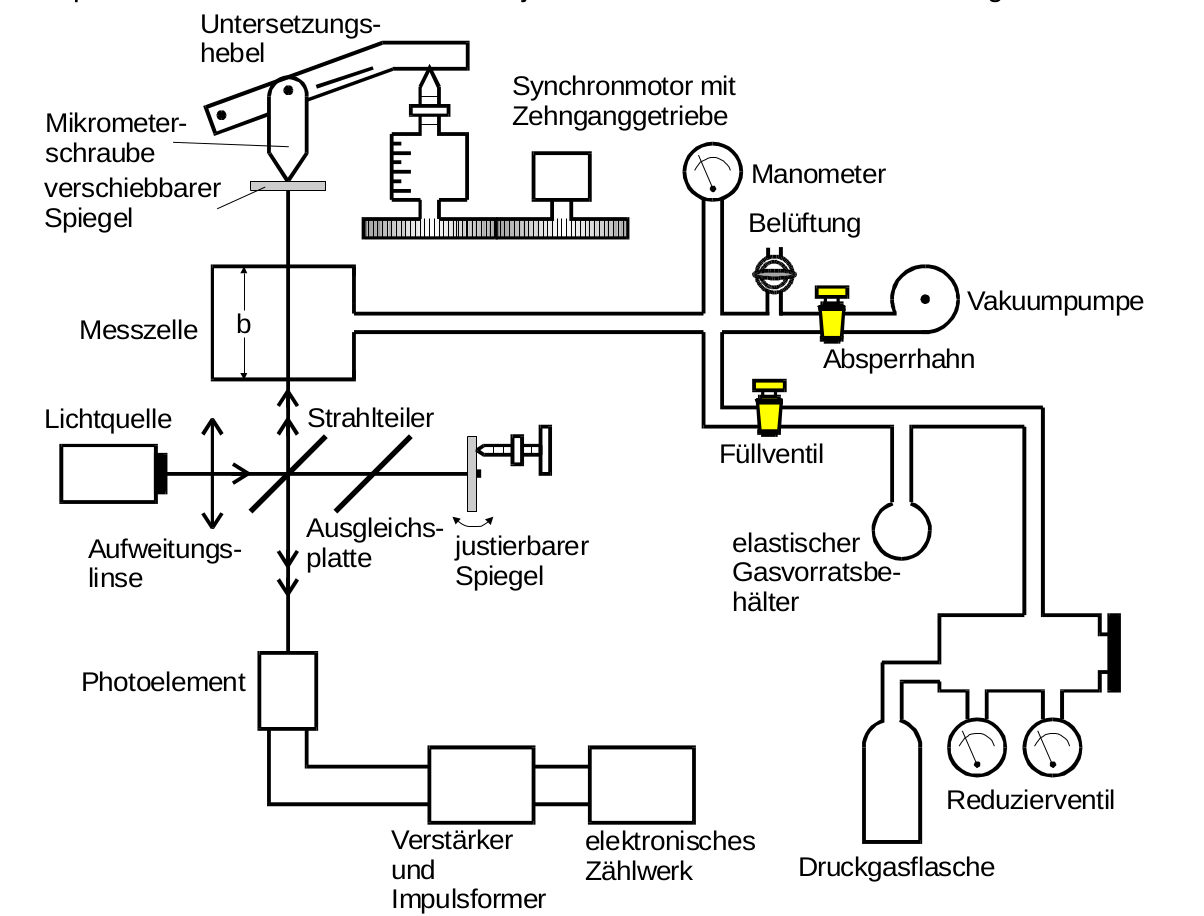
\includegraphics[width=0.72\textwidth]{Bilder/aufbau.png}
	\caption{Schematischer Aufbau der Messapparatur. \cite{Anleitung}}
  \label{fig:aufbau}
\end{figure}
Das Michelson-Interferometer ist wie in Abbildung \ref{fig:aufbau} aufgebaut.\\
Um Interferenzen beobachten zu können, wird der Laserstrahl zunächst durch einen Strahlteiler, realisiert als eine semipermeable Platte, in zwei Teilbündel aufgeteilt.

Für die spätere Messung ist einer der Strahlwege von variabler Länge. Dazu ist der Spiegel
des oberen Strahlwegs durch einen Synchronmotor mit Zehnganggetriebe verschiebbar.
\\Zusätzlich ist im oberen Strahlweg eine Messzelle mit Breite $b=\SI{50}{\milli\meter}$ installiert.
Diese lässt sich sowohl evakuieren, als auch mit verschiedenen Gasen befüllen, sodass durch den geänderten Brechungsindex in der Messzelle ebenso ein optischer Wegunterschied zwischen beiden Strahlwegen entsteht. \\
Im rechten Strahlweg ist zudem eine Ausgleichsplatte angebracht, da dieser Strahlweg im Gegensatz zum anderen Strahlweg nicht dreimal, sondern nur einmal durch den in der Mitte angebrachten Strahlteiler führt.
Beide Strahlwege treffen schließlich auf das Photoelement, an welchem die ankommenden Lichtsignale registriert werden und über einen Verstärker und einen Impulsformer an ein elektronisches Zählwerk gegeben wird.
